%!TEX program = xelatex
\documentclass[tikz,convert=pdf2svg]{standalone}
\usepackage{amsmath}
\usepackage{tikz}

\usetikzlibrary{shapes,backgrounds}
\usetikzlibrary{arrows, decorations.pathmorphing, backgrounds, positioning, fit, petri, automata} %自动机

\usetikzlibrary{matrix,arrows}

\begin{document}

    % \begin{tikzpicture}[>=latex, shorten >=1pt,node distance=0.75in, on grid, auto]
	% 	\node[state] (q0) {$q_0$};
	% 	\node[state,](q1) [below=of q0] {$q_1$};
	% 	\node[state,accepting] (q3) [below left=of q1] {$q_3$};
	% 	\node[state] (q2) [below right=of q1] {$q_2$};
	% 	\node[state] (q4) [below left=of q2] {$q_4$};
	% 	\node[state,initial] (s) [left=of q1] {$s$};
	% 	\node[state](dump) [above=of s] {$d$};
	% 	\path[->]
	% 	(s) edge node {$0$} (dump)
	% 	(s) edge node [bend left] {$1$} (q1)
	% 	(q0) edge [loop above] node {$0$} (q0)
	% 	(q0) edge [swap] node {$1$} (q1)
	% 	(q1) edge node {$0$} (q2)
	% 	(q2) edge node {$0$} (q4)
	% 	(q4) edge node {$0$} (q3)
	% 	(q3) edge [bend right,swap] node {$0$} (q1)
	% 	(q1) edge [swap] node {$1$} (q3)
	% 	(q2) edge [bend right] node {$1$} (q0)
	% 	(q3) edge [bend right] node {$1$} (q2)
	% 	(q4) edge [loop below] node {$1$} (q4)
    %     (dump) edge [loop above] node {$0,1$} (dump)
    %     ;
    %     \end{tikzpicture}
        

    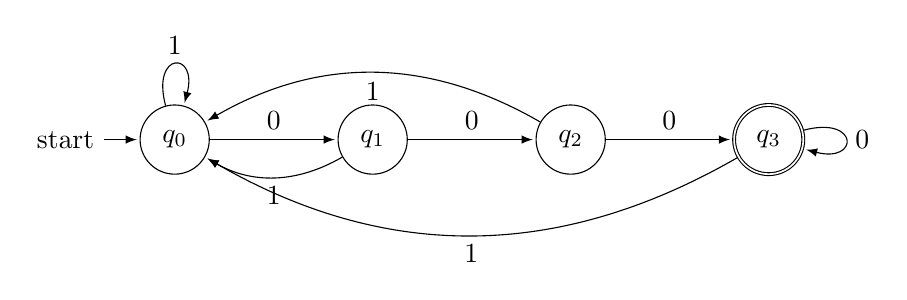
\begin{tikzpicture}[>=latex, shorten >=1pt,node distance=0.99in, on grid, auto]
        \node[state,initial] (q0) {$q_0$};
        \node[state] (q1) [right=of q0] {$q_1$};
        \node[state] (q2) [right=of q1] {$q_2$};
        \node[state,accepting] (q3) [right=of q2] {$q_3$};
        \path[->]
        (q0) edge node {$0$} (q1)
        (q1) edge node {$0$} (q2)
        (q2) edge node {$0$} (q3)
        (q1) edge [bend left] node {$1$} (q0)
        (q2) edge [bend right] node {$1$} (q0)
        (q3) edge [bend left] node {$1$} (q0)
        (q0) edge [loop above] node {$1$} (q0)
        (q3) edge [loop right] node {$0$} (q3)
        ;
    \end{tikzpicture}

    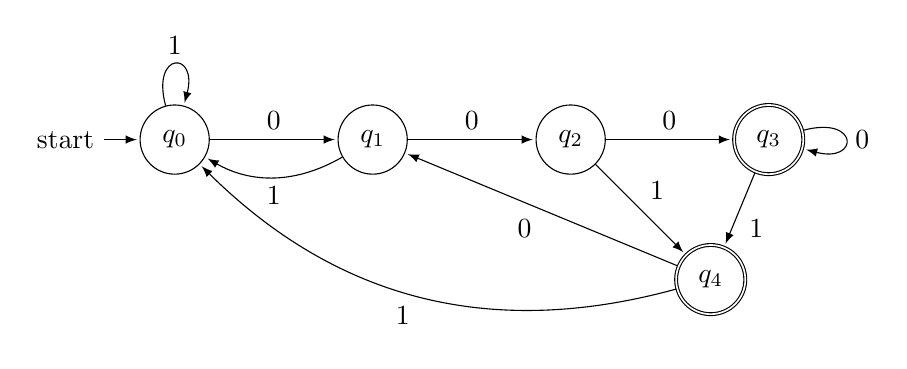
\begin{tikzpicture}[>=latex, shorten >=1pt,node distance=0.99in, on grid, auto]
        \node[state,initial] (q0) {$q_0$};
        \node[state] (q1) [right=of q0] {$q_1$};
        \node[state] (q2) [right=of q1] {$q_2$};
        \node[state,accepting] (q3) [right=of q2] {$q_3$};
        \node[state,accepting] (q4) [below right=of q2] {$q_4$};
        \path[->]
        (q0) edge node {$0$} (q1)
        (q1) edge node {$0$} (q2)
        (q2) edge node {$0$} (q3)
        (q1) edge [bend left] node {$1$} (q0)
        (q2) edge  node {$1$} (q4)
        (q3) edge  node {$1$} (q4)
        (q4) edge  node {$0$} (q1)
        (q0) edge [loop above] node {$1$} (q0)
        (q3) edge [loop right] node {$0$} (q3)
        (q4) edge [bend left] node {$1$} (q0)
        ;
    \end{tikzpicture}

    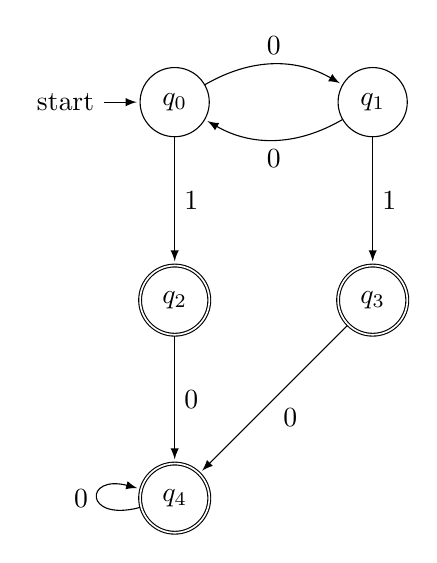
\begin{tikzpicture}[>=latex, shorten >=1pt,node distance=0.99in, on grid, auto]
        \node[state,initial] (q0) {$q_0$};
        \node[state] (q1) [right=of q0] {$q_1$};
        \node[state,accepting] (q2) [below=of q0] {$q_2$};
        \node[state,accepting] (q3) [right=of q2] {$q_3$};
        \node[state,accepting] (q4) [below=of q2] {$q_4$};
        \path[->]
        (q0) edge [bend left] node {$0$} (q1)
        (q1) edge [bend left] node {$0$} (q0)
        (q0) edge node {$1$} (q2)
        (q1) edge node {$1$} (q3)
        (q2) edge node {$0$} (q4)
        (q3) edge node {$0$} (q4)
        (q4) edge [loop left] node {$0$} (q4)
        ;
    \end{tikzpicture}



    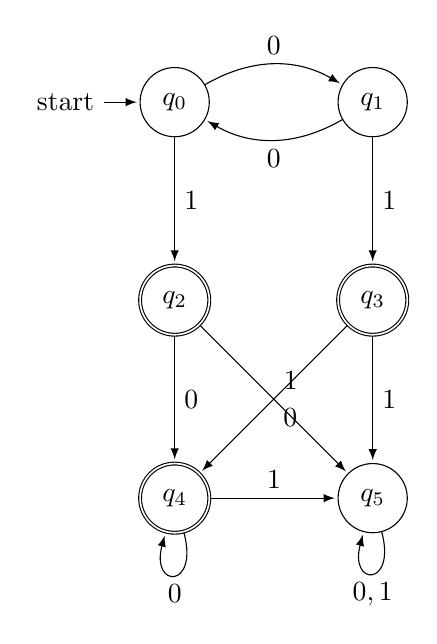
\begin{tikzpicture}[>=latex, shorten >=1pt,node distance=0.99in, on grid, auto]
        \node[state,initial] (q0) {$q_0$};
        \node[state] (q1) [right=of q0] {$q_1$};
        \node[state,accepting] (q2) [below=of q0] {$q_2$};
        \node[state,accepting] (q3) [right=of q2] {$q_3$};
        \node[state,accepting] (q4) [below=of q2] {$q_4$};
        \node[state] (q5) [right=of q4] {$q_5$};
        \path[->]
        (q0) edge [bend left] node {$0$} (q1)
        (q1) edge [bend left] node {$0$} (q0)
        (q0) edge node {$1$} (q2)
        (q1) edge node {$1$} (q3)
        (q2) edge node {$0$} (q4)
        (q2) edge node {$1$} (q5)
        (q3) edge node {$0$} (q4)
        (q3) edge node {$1$} (q5)
        (q4) edge [loop below] node {$0$} (q4)
        (q4) edge node {$1$} (q5)
        (q5) edge [loop below] node {$0,1$} (q5)
        ;
    \end{tikzpicture}




    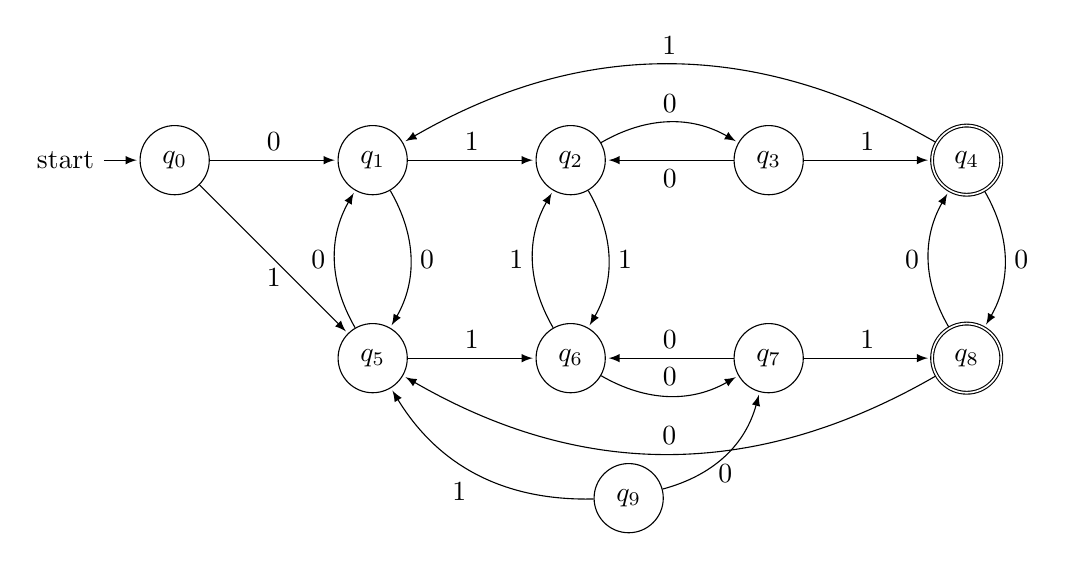
\begin{tikzpicture}[>=latex, shorten >=1pt,node distance=0.99in, on grid, auto]
        \node[state,initial] (q0) {$q_0$};
        \node[state] (q1) [right=of q0] {$q_1$};
        \node[state] (q2) [right=of q1] {$q_2$};
        \node[state] (q3) [right=of q2] {$q_3$};
        \node[state,accepting] (q4) [right=of q3] {$q_4$};
        \node[state] (q5) [below=of q1] {$q_5$};
        \node[state] (q6) [right=of q5] {$q_6$};
        \node[state] (q7) [right=of q6] {$q_7$};
        \node[state,accepting] (q8) [right=of q7] {$q_8$};
        \node[state] (q9) [below left=of q7] {$q_9$};
        \path[->]
        (q0) edge node {$0$} (q1)
        (q1) edge node {$1$} (q2)
        (q2) edge [bend left] node {$0$} (q3)
        (q3) edge node {$0$} (q2)
        (q3) edge node {$1$} (q4)
        (q5) edge node {$1$} (q6)
        (q6) edge [bend right] node {$0$} (q7)
        (q7) edge [above] node {$0$} (q6)
        (q7) edge node {$1$} (q8)
        (q8) edge [bend left,above] node {$0$} (q5)
        (q4) edge [bend right,above] node {$1$} (q1)
        (q1) edge [bend left] node {$0$} (q5)
        (q5) edge [bend left] node {$0$} (q1)
        (q2) edge [bend left] node {$1$} (q6)
        (q6) edge [bend left] node {$1$} (q2)
        (q4) edge [bend left] node {$0$} (q8)
        (q8) edge [bend left] node {$0$} (q4)
        (q9) edge [bend right,below] node {$0$} (q7)
        (q9) edge [bend left] node {$1$} (q5)
        (q0) edge [below] node {$1$} (q5)
        ;
    \end{tikzpicture}



    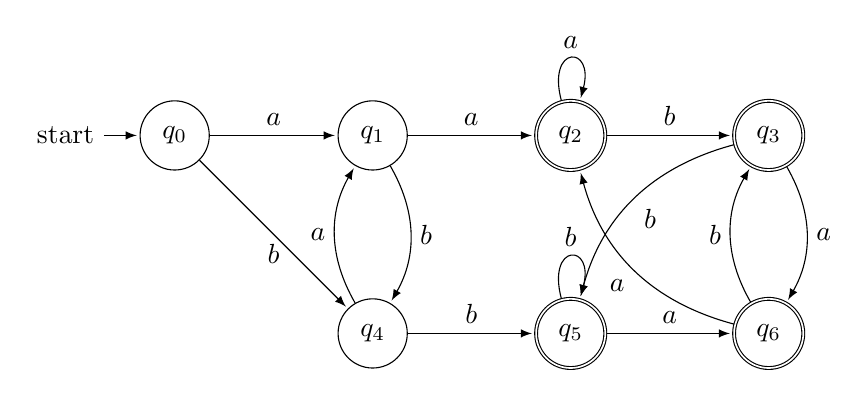
\begin{tikzpicture}[>=latex, shorten >=1pt,node distance=0.99in, on grid, auto]
        \node[state,initial] (q0) {$q_0$};
        \node[state] (q1) [right=of q0] {$q_1$};
        \node[state,accepting] (q2) [right=of q1] {$q_2$};
        \node[state,accepting] (q3) [right=of q2] {$q_3$};
        \node[state] (q4) [below=of q1] {$q_4$};
        \node[state,accepting] (q5) [right=of q4] {$q_5$};
        \node[state,accepting] (q6) [right=of q5] {$q_6$};
        \path[->]
        (q0) edge node {$a$} (q1)
        (q1) edge node {$a$} (q2)
        (q5) edge node {$a$} (q6)
        (q2) edge node {$b$} (q3)
        (q0) edge [below ]node {$b$} (q4)
        (q4) edge node {$b$} (q5)
        (q1) edge [bend left] node {$b$} (q4)
        (q4) edge [bend left] node {$a$} (q1)
        (q6) edge [bend left] node {$a$} (q2)
        (q3) edge [bend right] node {$b$} (q5)
        (q2) edge [loop above] node {$a$} (q2)
        (q5) edge [loop above] node {$b$} (q5)
        (q3) edge [bend left] node {$a$} (q6)
        (q6) edge [bend left] node {$b$} (q3)
        ;
    \end{tikzpicture}


\end{document}